%Preamble
\documentclass[12pt,a4paper]{article}
\usepackage[top=20mm, bottom=20mm, left=20mm, right=20mm]{geometry}
\usepackage[utf8]{inputenc}
\usepackage{fancyhdr} \setlength{\headheight}{15pt}
\usepackage{lastpage}
\usepackage{t1enc}
\usepackage[magyar]{babel}
\usepackage{amsmath}
\usepackage{amssymb,physics}
\usepackage{amsthm}
\usepackage{empheq}
\usepackage{enumitem}
\usepackage{subfiles}
\usepackage{float}
\usepackage{verbatim}
\usepackage{amsmath}
\usepackage{hyperref}
\usepackage{amsmath}
\usepackage{multicol}
\usepackage{tikz}
\usepackage{pgfplots}
\newcommand*\widefbox[1]{\fbox{\hspace{2em}#1\hspace{2em}}}
\pagestyle{fancy}
\def\mx#1{\mathbf{#1}}
\def\vec#1{\underline{\mathrm{#1}}}
\def\m{\; \left[\mathrm{m}\right]}
\def\deg{\; \left[^{\circ}\right]}
\def\mm{\; \left[\mathrm{m^2}\right]}
\def\i{\left(i\right)}
\def\cosalfa{\cos \alpha^{\i}}
\def\sinalfa{\sin \alpha^{\i}}
\def\cosalfasq{\cos^2 \alpha^{\i}}
\def\sinalfasq{\sin^2 \alpha^{\i}}
\def\Nm{\; \left[\mathrm{\frac{N}{m}}\right]}
\def\kN{\; \left[\mathrm{kN}\right]}
\def\futyi{\cdot 10^{7}}

\lhead{BMEGEMMBXVE, VEM alapjai 1. Szorgalmi HF}
\cfoot{\thepage\ / \pageref{LastPage}}
\rhead{Németh Áron Imre, D1J5ZG}

\begin{document}

\section{A szerkezet méretarányos ábrájának elkészítése}
\subsubsection*{Adatok:}
\begin{multicols}{2}
    \begin{itemize}
        \item $a=2 \m$
        \item $b=1.3 \m$
        \item $c=5 \m$
    \end{itemize}
    \columnbreak
    \begin{itemize}
        \item $d=50 \; \left[\mathrm{mm}\right]$
        \item $E=190 \; \left[\mathrm{GPa}\right]$
        \item $F=170 \; \kN$
    \end{itemize}
\end{multicols}
\subsubsection*{A szerkezet ábrája}
A szerkezet méretarányos ábrája esetünkben az alábbi módon néz ki:
\begin{figure}[H]
    \centering
    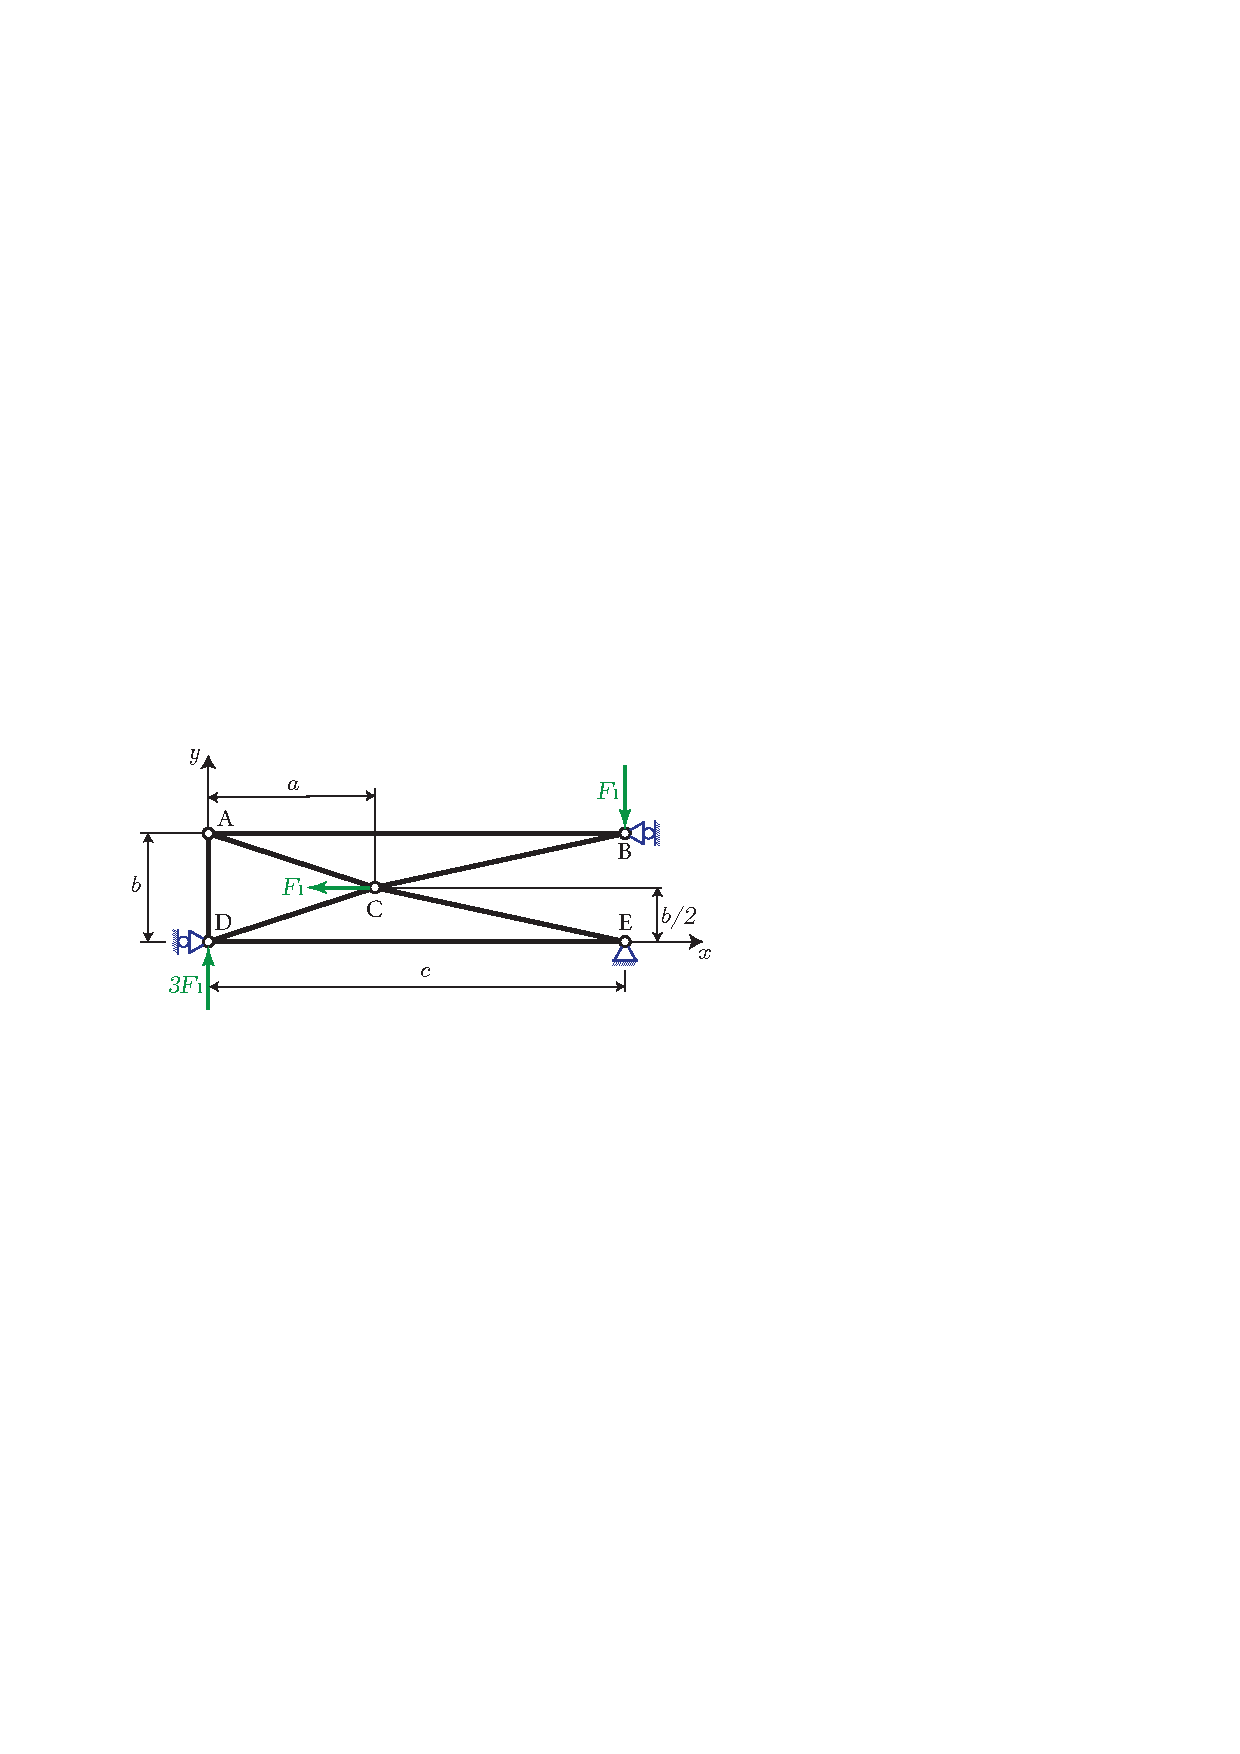
\includegraphics{vszhf1_abra.pdf}
    \caption{A szerkezet léptékhelyes ábrája}
\end{figure}
\section{Az elmozduláskomponensek meghatározása}
\subsection{A csomópontok definiálása}
Az alábbi táblázatban láthatóak a különböző csomópontok $x$ illetve
$y$ koordinátái:
\begin{center}
    \begin{tabular}{|c|c|c|}
        \hline
        Csomópont & x koordináta & y koordináta \\
        \hline
        \hline
        1         & 0            & b            \\
        \hline
        2         & c            & b            \\
        \hline
        3         & a            & b/2          \\
        \hline
        4         & 0            & 0            \\
        \hline
        5         & c            & 0            \\
        \hline
    \end{tabular}
\end{center}
\subsection{Elemek hozzárendelése a csomó pontokhoz}
Az alábbi táblázat tartalmazza a csomópont-elem hozzárendeléseket:
\begin{center}
    \begin{tabular}{|c|c|c|}
        \hline
        Elemszám & Lokális első csomópont & Lokális második csomópont \\
        \hline
        \hline
        1        & 1                      & 2                         \\
        \hline
        2        & 1                      & 3                         \\
        \hline
        3        & 2                      & 3                         \\
        \hline
        4        & 1                      & 4                         \\
        \hline
        5        & 3                      & 4                         \\
        \hline
        6        & 3                      & 5                         \\
        \hline
        7        & 4                      & 5                         \\
        \hline
    \end{tabular}
\end{center}
\subsection{Az elemi mennyiségek meghatározása}
\subsubsection{A rúdak hosszainak meghatározása}
A rúdak hosszait az alábbi általános képlet segítségével tudjuk
könnyen kiszámítani:
\begin{equation}
    \boxed{L^{\left(i\right)}=\sqrt{\left(x^{\left(i\right)}_2-x^{\left(i\right)}_1\right)^2+
            \left(y^{\left(i\right)}_2-y^{\left(i\right)}_1\right)^2}}
\end{equation}
Ezen képletet alkalmazva a rúdak hosszai numerikusan az alábbiak:
\begin{multicols}{4}
    \begin{itemize}
        \item $L_1=5 \m$
        \item $L_2=2.1029 \m$
    \end{itemize}
    \columnbreak
    \begin{itemize}
        \item $L_3=3.0696 \m$
        \item $L_4=1.3 \m$
    \end{itemize}
    \columnbreak
    \begin{itemize}
        \item $L_5=2.1029 \m$
        \item $L_6=3.0696 \m$
    \end{itemize}
    \columnbreak
    \begin{itemize}
        \item $L_7=5 \m$
    \end{itemize}
\end{multicols}
\subsubsection{A rúdak szöghelyzeteinek meghatározása}
A rúdak szöghelyzetét legegyszerűbben az alábbi általános összefüggés
segítségével számíthatjuk:
\begin{equation}
    \boxed{\alpha^{\left(i\right)}=
        \arctan \left( \frac{y^{\left(i\right)}_2-y^{\left(i\right)}_1}
        {x^{\left(i\right)}_2-x^{\left(i\right)}_1}\right)}
\end{equation}
Ez alapján a szögek numerikus értékei:
\begin{multicols}{3}
    \begin{itemize}
        \item $\alpha_1=\alpha_7=0 \deg$
        \item $\alpha_2=-18.004 \deg$
    \end{itemize}
    \columnbreak
    \begin{itemize}
        \item $\alpha_3=12.225 \deg$
        \item $\alpha_4=270 \deg$
    \end{itemize}
    \columnbreak
    \begin{itemize}
        \item $\alpha_5=18.004 \deg$
        \item $\alpha_6=-12.225 \deg$
    \end{itemize}
\end{multicols}
\subsubsection{Keresztmetszet jellemzőinek meghatározása}
Keresztmetszetünk esetünkben egy cső amelynek belső átmérője $d$, valamint falvastagsága
$0.15 d$, így ez alapján az alábbi módon számíthatjuk a csőszelvény területét:
\begin{equation}
    A=\frac{\left(\left(1.3 \cdot d\right)^2-d^2\right) \pi }
    {4}=0.00135 \mm
\end{equation}
\subsubsection{Az elemi merevségi mátrixok meghatározása}
Most hogy már ismerjük a rúdak hosszait, szöghelyzeteit valamint Keresztmetszetét,
az alábbi 2D-s húzott-nyomott rúdelemre vonatkozó összefüggéssel meghatározhatjuk a
különböző elemek merevségi mátrixait.
\begin{equation}
    \mx{K}^{\i}=\frac{A \; E}{L^{\i}}
    \begin{bmatrix}
        \cosalfasq          &  & \cosalfa \sinalfa   &  & -\cosalfasq          &  & - \cosalfa  \sinalfa \\
        \cosalfa  \sinalfa  &  & \sinalfasq          &  & - \cosalfa  \sinalfa &  & -\sinalfasq          \\
        -\cosalfasq         &  & -\cosalfa  \sinalfa &  & \cosalfasq           &  & \cosalfa  \sinalfa   \\
        -\cosalfa  \sinalfa &  & -\sinalfasq         &  & \cosalfa  \sinalfa   &  & \sinalfasq           \\
    \end{bmatrix}
\end{equation}
\subsubsection*{Így az elemi merevségi mátrixok:}
\begin{equation}
    \mx{K}^{\left(1\right)}=\mx{K}^{\left(7\right)}=
    \begin{bmatrix}
        5.1482 \futyi  &  & 0 &  & -5.1482 \futyi &  & 0      \\
        0              &  & 0 &  & 0              &  & 0 &  & \\
        -5.1482 \futyi &  & 0 &  & 5.1482 \futyi  &  & 0      \\
        0              &  & 0 &  & 0              &  & 0 &  &
    \end{bmatrix} \Nm
\end{equation}
\begin{equation}
    \mx{K}^{\left(2\right)}=
    \begin{bmatrix}
        11.0711 \futyi  &  & -3.5981 \futyi &  & -11.0711 \futyi &  & 3.5981 \futyi  \\
        -3.5981 \futyi  &  & 1.1693 \futyi  &  & 3.5981 \futyi   &  & -1.1693 \futyi \\
        -11.0711 \futyi &  & 3.5981 \futyi  &  & 11.0711 \futyi  &  & -3.5981 \futyi \\
        3.5981 \futyi   &  & -1.1693 \futyi &  & -3.5981 \futyi  &  & 1.1693 \futyi
    \end{bmatrix} \Nm
\end{equation}
\begin{equation}
    \mx{K}^{\left(3\right)}=
    \begin{bmatrix}
        8.0098 \futyi  &  & 1.7354 \futyi  &  & -8.0098 \futyi &  & -1.7354 \futyi \\
        1.7354 \futyi  &  & 0.3760 \futyi  &  & -1.7354 \futyi &  & -0.3760 \futyi \\
        -8.0098 \futyi &  & -1.7354 \futyi &  & 8.0098 \futyi  &  & 1.7354 \futyi  \\
        -1.7354 \futyi &  & -0.3760 \futyi &  & 1.7354 \futyi  &  & 0.3760 \futyi
    \end{bmatrix} \Nm
\end{equation}
\begin{equation}
    \mx{K}^{\left(4\right)}=
    \begin{bmatrix}
        0 &  & 0               &  & 0 &  & 0              \\
        0 &  & 19.8011 \futyi  &  & 0 &  & -19.801 \futyi \\
        0 &  & 0               &  & 0 &  & 0              \\
        0 &  & -19.8011 \futyi &  & 0 &  & 19.801 \futyi
    \end{bmatrix} \Nm
\end{equation}
\begin{equation}
    \mx{K}^{\left(5\right)}=
    \begin{bmatrix}
        11.0711 \futyi  &  & 3.5981 \futyi  &  & -11.0711 \futyi &  & -3.5981 \futyi \\
        3.5981 \futyi   &  & 1.1693 \futyi  &  & -3.5981 \futyi  &  & -1.1693 \futyi \\
        -11.0711 \futyi &  & -3.5981 \futyi &  & 11.0711 \futyi  &  & 3.5981 \futyi  \\
        -3.5981 \futyi  &  & -1.1693 \futyi &  & 3.5981 \futyi   &  & 1.1693 \futyi
    \end{bmatrix} \Nm
\end{equation}
\begin{equation}
    \mx{K}^{\left(6\right)}=
    \begin{bmatrix}
        8.0098 \futyi  &  & -1.7354 \futyi &  & -8.0098 \futyi &  & 1.7354 \futyi  \\
        -1.7354 \futyi &  & 0.3760 \futyi  &  & 1.7354 \futyi  &  & -0.3760 \futyi \\
        -8.0098 \futyi &  & 1.7354 \futyi  &  & 8.0098 \futyi  &  & -1.7354 \futyi \\
        1.7354 \futyi  &  & -0.3760 \futyi &  & -1.7354 \futyi &  & 0.3760 \futyi
    \end{bmatrix} \Nm
\end{equation}
\subsubsection{Elemi elmozdulásvektorok meghatározása}
Az elemi elmozdulásvektor alakja minden esetben az alábbi módon néz ki:
\begin{equation}
    \vec{\mathbf{U}}^{\i}=
    \begin{bmatrix}
        {u_1}^{\i} \\
        {v_1}^{\i} \\
        {u_2}^{\i} \\
        {v_2}^{\i}
    \end{bmatrix}
\end{equation}
Ahol:
\begin{itemize}
    \item A felső index az rúdelemre utal
    \item Az alsó indexek pedig a lokális csomópontokra
\end{itemize}
\subsubsection*{Peremfeltételek:}
\begin{itemize}
    \item  Mivel az $\left(1\right)$-es csomópont nincs semmilyen módon
          befogva, így mindkét irányú elmozduláskomponens ébred.
    \item A  $\left(2\right)$-es csomópont görgős csuklóval van rögzítve, így
          csak $y$ irányú elmozduláskomponens ébred. $\; \rightarrow \; \boxed{u_{2}=0 \m}$
    \item A  $\left(3\right)$-as csomópont nincs befogva, így ebben az esetben is mindkét
          irányú elmozduláskomponensünk van.
    \item A $\left(4\right)$-es csomópont is görgős csuklóval van rögzítve
          így csak $y$ irányú elmozduláskomponens ébred. $\; \rightarrow \; \boxed{u_{4}=0 \m}$
    \item Az $\left(5\right)$-ös csomópont csuklóval van befogva, így egyik irányban sem történik
          elmozdulás. $\; \rightarrow \; \boxed{u_{5}=v_{5}=0 \m}$
\end{itemize}
Így az elemi elmozdulásvektorok:
\begin{multicols}{7}
    \noindent
    \begin{equation*}
        \vec{U}^{\left(1\right)}=
        \begin{bmatrix}
            u_1 \\
            v_1 \\
            0   \\
            v_2
        \end{bmatrix}
    \end{equation*}
    \columnbreak
    \begin{equation*}
        \vec{U}^{\left(2\right)}=
        \begin{bmatrix}
            u_1 \\
            v_1 \\
            u_3 \\
            v_3
        \end{bmatrix}
    \end{equation*}
    \columnbreak
    \begin{equation*}
        \vec{U}^{\left(3\right)}=
        \begin{bmatrix}
            0   \\
            v_2 \\
            u_3 \\
            v_3
        \end{bmatrix}
    \end{equation*}
    \columnbreak
    \begin{equation*}
        \vec{U}^{\left(4\right)}=
        \begin{bmatrix}
            u_1 \\
            v_1 \\
            0   \\
            v_4
        \end{bmatrix}
    \end{equation*}
    %\end{multicols}
    %\begin{multicols}{3}
    %    \noindent
    \begin{equation*}
        \vec{U}^{\left(5\right)}=
        \begin{bmatrix}
            u_3 \\
            v_3 \\
            0   \\
            v_4
        \end{bmatrix}
    \end{equation*}
    \columnbreak
    \begin{equation*}
        \vec{U}^{\left(6\right)}=
        \begin{bmatrix}
            u_3 \\
            v_3 \\
            0   \\
            0
        \end{bmatrix}
    \end{equation*}
    \columnbreak
    \begin{equation*}
        \vec{U}^{\left(7\right)}=
        \begin{bmatrix}
            u_4 \\
            v_4 \\
            0   \\
            0
        \end{bmatrix}
    \end{equation*}
\end{multicols}
\subsubsection{Elemi terhelésvektorok meghatározása}
Az elemi terhelésvektor alakja minden esetben az alábbi módon néz ki:
\begin{equation}
    \vec{F}^{\i}=
    \begin{bmatrix}
        F_{1x}^{\i} \\
        F_{1y}^{\i} \\
        F_{2x}^{\i} \\
        F_{2y}^{\i}
    \end{bmatrix}
\end{equation}
\subsubsection*{Peremfeltételek:}
\begin{itemize}
    \item Mivel az $\left(1\right)$-es csomópont nincs semmilyen módon
          befogva, valamint nem hat rá aktív terhelés, így a benne fellépő
          reakcióerők zérusok. $\; \rightarrow \; \boxed{F_{x_1}=F_{y_1}= 0 \kN}$
    \item A  $\left(2\right)$-es csomópont görgős csuklóval van rögzítve, így
          csak $x$ irányú reakcióerő ébred, valamint az $y$ irányú terhelést már ismerjük.
          $\; \rightarrow \; \boxed{F_{y_2}=-F=-170 \kN}$
    \item A  $\left(3\right)$-as csomópont nincs befogva, valamint egy $x$
          irányú aktív terhelés hat rá, így tehát $\; \rightarrow \; \boxed{F_{x_3}=-F=-170 \kN \hspace{5mm}
                  F_{y_3}=0 \kN}$
    \item A $\left(4\right)$-es csomópont is görgős csuklóval van rögzítve,
          így csak $x$ irányú reakcióerő ébred, valamint az $y$ irányú aktív
          terhelést ismerjük. $\; \rightarrow \; \boxed{F_{y_4}=3 F=510 \kN}$
    \item Az $\left(5\right)$-ös csomópont csuklóval van befogva, így mindkét irányú
          reakcióerő ébred.
\end{itemize}
Így az elemi terhelésvektorok:
\begin{multicols}{7}
    \noindent
    \begin{equation*}
        \vec{F}^{\left(1\right)}=
        \begin{bmatrix}
            0       \\
            0       \\
            F_{x_2} \\
            -F
        \end{bmatrix}
    \end{equation*}
    \columnbreak
    \begin{equation*}
        \vec{F}^{\left(2\right)}=
        \begin{bmatrix}
            0  \\
            0  \\
            -F \\
            0
        \end{bmatrix}
    \end{equation*}
    \columnbreak
    \begin{equation*}
        \vec{F}^{\left(3\right)}=
        \begin{bmatrix}
            F_{x_2} \\
            -F      \\
            -F      \\
            0
        \end{bmatrix}
    \end{equation*}
    \columnbreak
    \begin{equation*}
        \vec{F}^{\left(4\right)}=
        \begin{bmatrix}
            0       \\
            0       \\
            F_{x_4} \\
            3 F
        \end{bmatrix}
    \end{equation*}
    %\end{multicols}
    %\begin{multicols}{3}
    %    \noindent
    \begin{equation*}
        \vec{F}^{\left(5\right)}=
        \begin{bmatrix}
            -F      \\
            0       \\
            F_{x_4} \\
            3 F
        \end{bmatrix}
    \end{equation*}
    \columnbreak
    \begin{equation*}
        \vec{F}^{\left(6\right)}=
        \begin{bmatrix}
            -F      \\
            0       \\
            F_{x_5} \\
            F_{y_5}
        \end{bmatrix}
    \end{equation*}
    \columnbreak
    \begin{equation*}
        \vec{F}^{\left(7\right)}=
        \begin{bmatrix}
            F_{x_4} \\
            3 F     \\
            F_{x_5} \\
            F_{y_5}
        \end{bmatrix}
    \end{equation*}
\end{multicols}
\subsection{Globális mennyiségek meghatározása}
\subsubsection{Globális merevségi mátrix meghatározása}
\subsubsection{Globális elmozdulásvektor és terhelésvektor meghatározása}
A globális elmozdulásvektor és terhelésvektor az alábbi módon néznek ki, a peremfeltételeket
figyelembe véve:
\begin{multicols}{2}
    \noindent
    \begin{equation}
        \vec{\mathbf{U}}=
        \begin{bmatrix}
            u_1 \\
            v_1 \\
            0   \\
            v_2 \\
            u_3 \\
            v_3 \\
            0   \\
            v_4 \\
            0   \\
            0
        \end{bmatrix}
    \end{equation}
    \columnbreak
    \begin{equation}
        \vec{\mathbf{F}}=
        \begin{bmatrix}
            0       \\
            0       \\
            F_{x_2} \\
            -F      \\
            -F      \\
            0       \\
            F_{x_4} \\
            3 F     \\
            F_{x_5} \\
            F_{y_5}
        \end{bmatrix}
    \end{equation}
\end{multicols}

\newpage
\tableofcontents

\end{document}